\documentclass[a4paper]{article}
\usepackage{amsfonts}
\usepackage{amsmath}
\usepackage{amssymb}
\usepackage{graphicx}     

\begin{document}
  
\noindent \large Auteur: Noran Ben Said \\
\noindent \large Studierichting: Informatica\\
\noindent \large Oefeningenreeks 5D nr. 1.6 \\
\medskip

\normalsize

$f(x) = \dfrac{x}{x^2-1} \text{ op } \left[-\dfrac{1}{2},\dfrac{1}{3}\right]$\\

$S = \displaystyle \int_a^b |f(x)|dx $\\

$S = \displaystyle \int_{-\tfrac{1}{2}}^0 \dfrac{x}{x^2-1}\,dx 
- \displaystyle \int_0^{\tfrac{1}{3}} \dfrac{x}{x^2-1}\,dx$\\

Stel $ u = x^2 - 1$\\

$du = 2x\,dx \Rightarrow x\,dx = \dfrac{1}{2}du$\\

$\displaystyle\int \dfrac{x}{x^2-1}\,dx 
=\dfrac{1}{2}\displaystyle\int \dfrac{1}{u}\,du$\\

$= \dfrac{1}{2}\ln|u|$\\

$= \dfrac{1}{2}\ln|x^2-1|$\\

Dus:\\

$S = \left[\dfrac{1}{2}\ln|x^2-1|\right]_{-\tfrac{1}{2}}^0
-
\left[\dfrac{1}{2}\ln|x^2-1|\right]_0^{\tfrac{1}{3}}$\\

$= \dfrac{1}{2}\ln\dfrac{3}{2}$\\

\begin{figure}[h]
\centering
    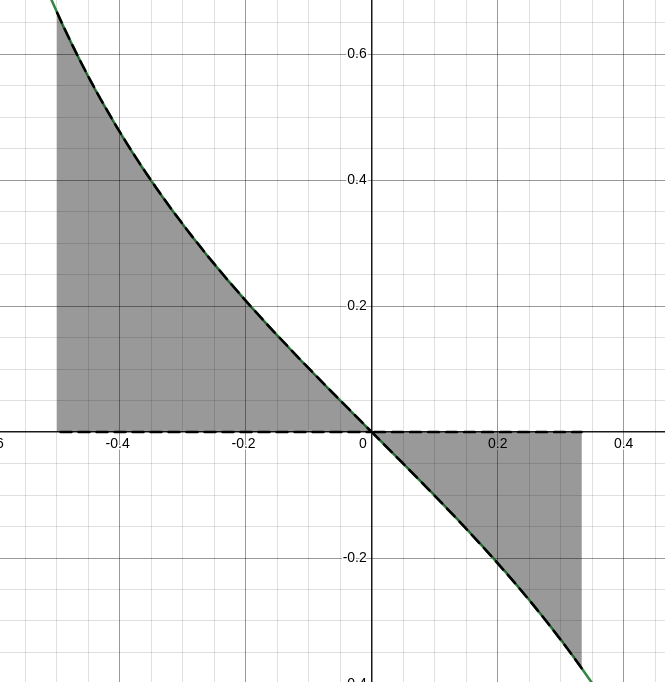
\includegraphics[width=5cm]{5D-1.6-noran.ben.said.ouald.abdelkarim.INF.png}\\
\end{figure}


\begin{thebibliography}{999}
%\bibitem{a} Referentie
\end{thebibliography}
\end{document} 

